\let\lesson\undefined
\newcommand{\lesson}{\phantomlesson{Bài 6: Định luật Boyle. Định luật Charles}}
\chapter[Định luật Boyle]{Định luật Boyle}
\section{Lý thuyết}
\subsection{Trạng thái và quá trình biến đổi trạng thái}
\begin{description}
	\item[Trạng thái của một khối khí] được xác định bằng ba thông số, gọi là thông số trạng thái của khối khí: thể tích $V$, áp suất $p$ và nhiệt độ tuyệt đối $T$. Giữa các thông số trạng thái của một khối khí xác định có những mối liên hệ mang tính quy luật.
	\begin{center}
		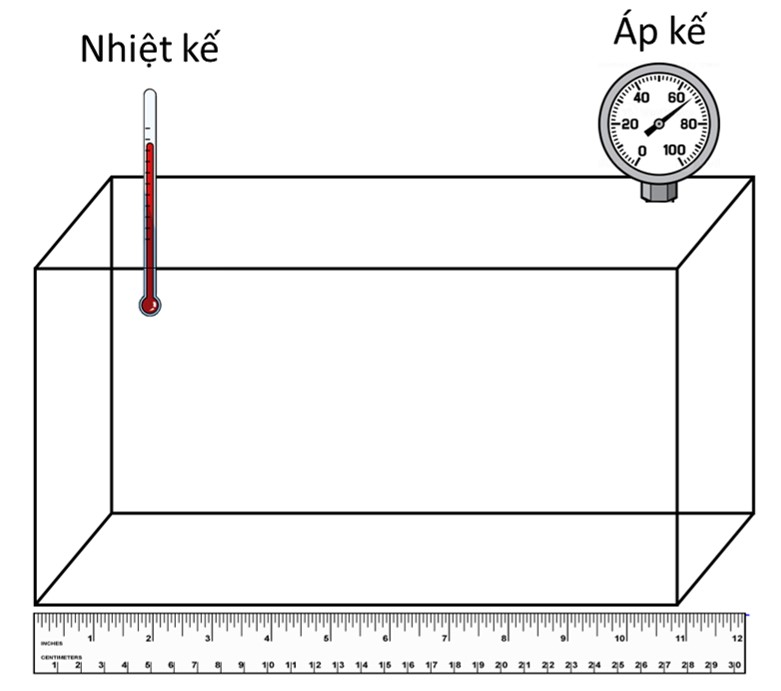
\includegraphics[width=0.35\linewidth]{../figs/VN12-Y24-PH-SYL-010-1}
		\captionof{figure}{Xác định các thông số trạng thái của một lượng khí.}
	\end{center}
	\item[Quá trình biến đổi trạng thái là] quá trình khối khí biến đổi từ trạng thái này sang trạng thái khác.
	\item[Đẳng quá trình] là quá trình biến đổi trạng thái mà trong đó có một thông số trạng thái được giữ không đổi.
\end{description}
Các đẳng quá trình:
\begin{itemize}
	\item Đẳng nhiệt là quá trình biến đổi trạng thái của một khối khí xác định, trong đó nhiệt độ được giữ không đổi.
	\item Đẳng áp là quá trình biến đổi trạng thái của một khối khí xác định, trong đó áp suất được giữ không đổi.
	\item Đẳng tích là quá trình biến đổi trạng thái của một khối khí xác định, trong đó thể tích được giữ không đổi.
\end{itemize}


\luuy{Vì chất khí luôn chiếm toàn bộ dung tích của bình chứa nên thể tích của một lượng khí bằng dung tích bình chứa nó.}
\subsection{Định luật Boyle}
Ở nhiệt độ không đổi, áp suất của một khối khí xác định tỉ lệ nghịch với thể tích của nó.
\begin{equation}
	pV=\text{hằng số}
\end{equation}
Đường biểu diễn sự phụ thuộc của $p$ theo $V$ khi nhiệt độ của khối khí không đổi gọi là \textbf{đường đẳng nhiệt}.
\begin{center}
	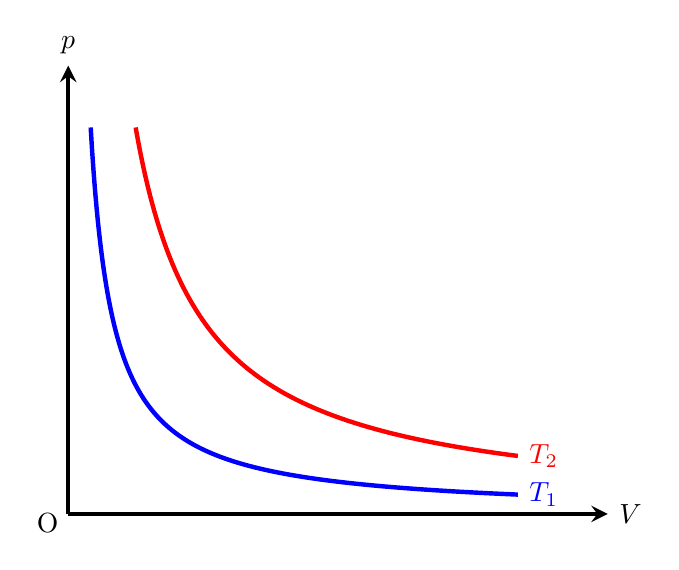
\begin{tikzpicture}  
		\begin{axis}[  ultra thick,
			xmin=0,  
			xmax=24,  
			xtick=\empty,
			ytick=\empty,
			ymin=0,  
			ymax=5.8, 
			samples=300,
			xticklabels=\empty,
			yticklabels=\empty,
			axis lines=center, 
			xlabel=$V$, 
			ylabel=$p$, 
			every axis y label/.style={at=(current axis.above origin),anchor=south},  
			every axis x label/.style={at=(current axis.right of origin),anchor=west},  ]
			\addplot [ultra thick, blue, smooth, domain=1:20] {5/x} node[right] {$T_1$}; 
			\addplot [ultra thick, red, smooth, domain=3:20] {15/x} node[right] {$T_2$}; 
		\end{axis}  
	\node[label={[below left]90:O}] at (0,0){};
	\end{tikzpicture}
\captionof{figure}{Các đường đẳng nhiệt của một khối khí lí tưởng tương ứng với nhiệt độ $T_1$ và $T_2\left(T_2>T_1\right)$.}
	
\end{center}
\section{Mục tiêu bài học - Ví dụ minh hoạ}
\begin{dang}{Vận dụng định luật Boyle giải thích được một số hiện tượng trong thực tế.}
	\viduii{2}
	{Nếu lật úp một chiếc cốc thuỷ tinh rồi nhúng chìm chiếc cốc vào trong nước thì thể tích phần không khí bị giam trong cốc sẽ thay đổi như thế nào trong quá trình chiếc cốc chìm sâu xuống nước?
	
}
{\hide{
	Trong quá trình cốc chìm xuống nước thì nhiệt độ không khí trong cốc không thay đổi. Cốc càng chìm sâu vào trong nước thì áp suất của không khí trong cốc càng tăng. Theo định luật Boyle, khi đó thể tích của không khí bị giam trong cốc ngày càng giảm.
}
}
	
	\viduii{2}
	{Để đưa thuốc từ lọ vào trong cylanh của ống tiêm, ban đầu nhân viên y tế đẩy piston sát đáy cylanh, sau đó đưa đầu kim tiêm (được gắn với ống tiêm) vào trong lọ thuốc. Khi kéo piston, thuốc sẽ chảy vào trong cylanh. Em hãy giải thích cơ sở khoa học của việc làm trên?
		\begin{center}
			
\includegraphics[width=0.35\linewidth]{../figs/VN12-Y24-PH-SYL-010-2}
		\end{center}
	
}
{\hide{
	Khi mới đưa đầu kim tiêm vào trong lọ thuốc, áp suất khí còn lại trong cylanh bằng áp suất chất lỏng trong lo thuốc. Khi kéo piston, thể tích khí trong cylanh tăng (nhiệt độ khí gần như không đổi). Theo định luật Boyle, áp suất khí trong cylanh giảm và nhỏ hơn áp suất chất lỏng trong lọ. Do đó, chất lỏng trong lọ bị đẩy qua kim và chảy sang cylanh cho đến khi có sự cân bằng áp suất ở cả hai phía.
}
}
	
\end{dang}
\begin{dang}{Giải được các bài toán liên quan quá trình đẳng nhiệt}
	\viduii{2}
	{Một lượng khí có thể tích $\SI{10}{\text{lít}}$ ở áp suất $\SI{E5}{\pascal}$. Tính thể tích của lượng khí này ở áp suất $\SI{1.25E5}{\pascal}$. Biết nhiệt độ của khí không đổi.
	
}
{\hide{
	\begin{center}
		\begin{tabular}{C{4cm} C{3cm} C{4cm}}
			\colorbox{yellow}{\textcolor{red}{\textbf{Trạng thái 1}}} & $\xrightarrow[]{T_1=T_2}$ & \colorbox{yellow}{\textcolor{red}{\textbf{Trạng thái 2}}}\\
			$p_1=\SI{E5}{\pascal}$ & &$p_2=\SI{1.25E5}{\pascal}$\\
			$V_1=\SI{10}{\text{lít}}$ & & $V_2=?$
		\end{tabular}
	\end{center}
Theo định luật Boyle:
$$p_1V_1=p_2V_2\Rightarrow V_2=\dfrac{p_1V_1}{p_2}=\dfrac{\left(\SI{E5}{\pascal}\right)\cdot\left(\SI{10}{\text{lít}}\right)}{\SI{1.25E5}{\pascal}}=\SI{8}{\text{lít}}.$$
Vậy: ở áp suất $\SI{1.25E5}{\pascal}$ thì thể tích bọt khí là $\SI{8}{\text{lít}}$.
}}

\viduii{3}
{Một bọt khí nổi lên từ đáy giếng sâu $\SI{6}{\meter}$ lên mặt nước. Khi lên tới mặt nước, thể tích của bọt khí tăng lên bao nhiêu lần? Coi áp suất khí quyển là $\SI{1.013E5}{\pascal}$; khối lượng riêng của nước giếng là $\SI{1003}{\kilogram/\meter^3}$ và nhiệt độ của nước giếng không thay đổi theo độ sâu. Lấy gia tốc trọng trường $g=\SI{9.81}{\meter/\second^2}$.

}
{\hide{
Áp suất trong bọt khí khi ở độ sâu $\SI{6}{\meter}$ so với mặt nước:
	$$p_1=p_0+\rho gh=\SI{1.013E5}{\pascal}+\left(\SI{1003}{\kilogram/\meter^3}\right)\cdot\left(\SI{9.81}{\meter
		/\second^2}\right)\cdot\left(\SI{6}{\meter}\right)\approx\SI{1.6E5}{\pascal}$$
	\begin{center}
		\begin{tabular}{C{4cm} C{3cm} C{4cm}}
			\colorbox{yellow}{\textcolor{red}{\textbf{Trạng thái 1}}} & $\xrightarrow[]{T_1=T_2}$ & \colorbox{yellow}{\textcolor{red}{\textbf{Trạng thái 2}}}\\
			$p_1=\SI{1.6E5}{\pascal}$ & &$p_2=p_0=\SI{1.013E5}{\pascal}$\\
			$V_1$ & & $V_2$
		\end{tabular}
	\end{center}
Theo định luật Boyle:
$$p_1V_1=p_2V_2\Rightarrow \dfrac{V_2}{V_1}=\dfrac{p_1}{p_2}=\dfrac{\SI{1.6E5}{\pascal}}{\SI{1.013E5}{\pascal}}\approx1,58.$$
Vậy: khi nổi lên mặt nước, thể tích bọt khí đã tăng lên 1,58 lần.
}}

\viduii{4}
{Một cột không khí chứa trong một ống nhỏ, dài, tiết diện đều, ban đầu ống được đặt nằm ngang (như hình). Cột không khí được ngăn cách bởi một cột thuỷ ngân có chiều dài $d=\SI{150}{\milli\meter}$. Áp suất khí quyển là $p_0=\SI{750}{\milli\meter Hg}$. Biết chiều dài ban đầu của cột không khí là $\ell_0=\SI{144}{\milli\meter}$.
	\begin{center}
		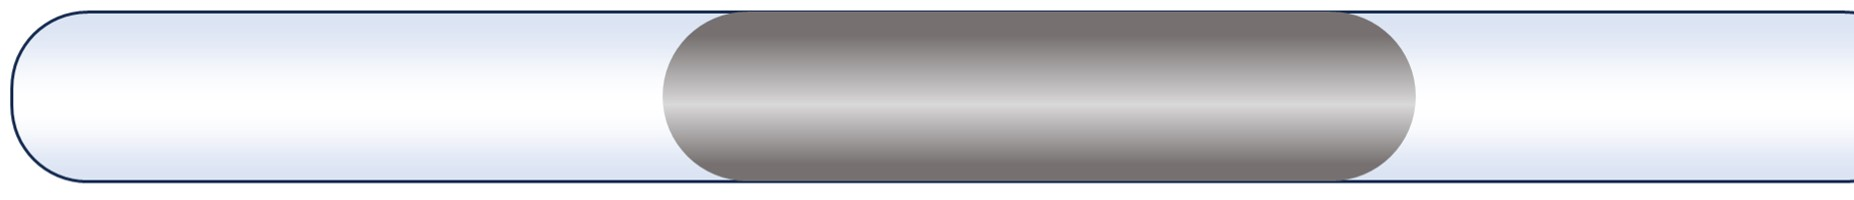
\includegraphics[width=0.4\linewidth]{../figs/VN12-Y24-PH-SYL-010-3}
	\end{center}
Hãy tính chiều dài cột không khí nếu:
\begin{enumerate}[label=\alph*)]
	\item ống thẳng đứng, miệng ống ở trên.
	\item ống thẳng đứng, miệng ống ở dưới.
	\item ống đặt nghiêng góc $\alpha=\SI{30}{\degree}$ so với phương ngang, miệng ống ở dưới.
	\item ống đặt nghiêng góc $\alpha=\SI{30}{\degree}$ so với phương ngang, miệng ống ở trên.
\end{enumerate}
Giả sử ống đủ dài để cột thuỷ ngân luôn ở trong ống và nhiệt độ là không đổi.
}
{\hide{Gọi $S$ là tiết diện của ống.
	\begin{enumerate}[label=\alph*)]
		\item Trường hợp ống đặt thẳng đứng, miệng ống hướng lên:\\
\begin{minipage}[l]{0.25\textwidth}
	\begin{center}
		
\includegraphics[width=0.1\linewidth]{../figs/VN12-Y24-PH-SYL-010-4}
	\end{center}
\end{minipage}
\begin{minipage}[l]{0.75\textwidth}
	\begin{center}
		\begin{tabular}{C{4cm} C{2cm} C{4cm}}
			\colorbox{yellow}{\textcolor{red}{\textbf{Trạng thái ban đầu}}} & $\xrightarrow[]{T=const}$ & \colorbox{yellow}{\textcolor{red}{\textbf{Trạng thái câu a}}}\\
			$p_0=\SI{750}{\milli\meter Hg}$ & &$p_a=p_0+d=\SI{900}{\milli\meter Hg}$\\
			$V_0=\ell_0S$ & & $V_a=\ell_a S$
		\end{tabular}
	\end{center}
	Theo định luật Boyle:
	$$p_0V_0=p_aV_a$$
	$$\Leftrightarrow p_0\ell_0S=p_a\ell_aS$$
	$$\Rightarrow \ell_a=\dfrac{p_0\ell_0}{p_a}=\dfrac{\left(\SI{750}{\milli\meter Hg}\right)\cdot\left(\SI{144}{\milli\meter}\right)}{\SI{900}{\milli\meter Hg}}=\SI{120}{\milli\meter}.$$
\end{minipage}
\item Trường hợp ống đặt thẳng đứng, miệng ống hướng xuống:\\
\begin{minipage}[l]{0.25\textwidth}
	\begin{center}
		
\includegraphics[width=0.1\linewidth]{../figs/VN12-Y24-PH-SYL-010-5}
	\end{center}
\end{minipage}
\begin{minipage}[l]{0.75\textwidth}
	\begin{center}
		\begin{tabular}{C{4cm} C{2cm} C{4cm}}
			\colorbox{yellow}{\textcolor{red}{\textbf{Trạng thái ban đầu}}} & $\xrightarrow[]{T=const}$ & \colorbox{yellow}{\textcolor{red}{\textbf{Trạng thái câu b}}}\\
			$p_0=\SI{750}{\milli\meter Hg}$ & &$p_b=p_0-d=\SI{600}{\milli\meter Hg}$\\
			$V_0=\ell_0S$ & & $V_b=\ell_b S$
		\end{tabular}
	\end{center}
	Theo định luật Boyle:
	$$p_0V_0=p_bV_b$$
	$$\Leftrightarrow p_0\ell_0S=p_b\ell_bS$$
	$$\Rightarrow \ell_b=\dfrac{p_0\ell_0}{p_b}=\dfrac{\left(\SI{750}{\milli\meter Hg}\right)\cdot\left(\SI{144}{\milli\meter}\right)}{\SI{600}{\milli\meter Hg}}=\SI{180}{\milli\meter}.$$
\end{minipage}
\item Trường hợp ống đặt nghiêng góc $\alpha=\SI{30}{\degree}$ so với phương ngang, miệng ống ở dưới:\\
\begin{minipage}[l]{0.25\textwidth}
	\begin{center}
		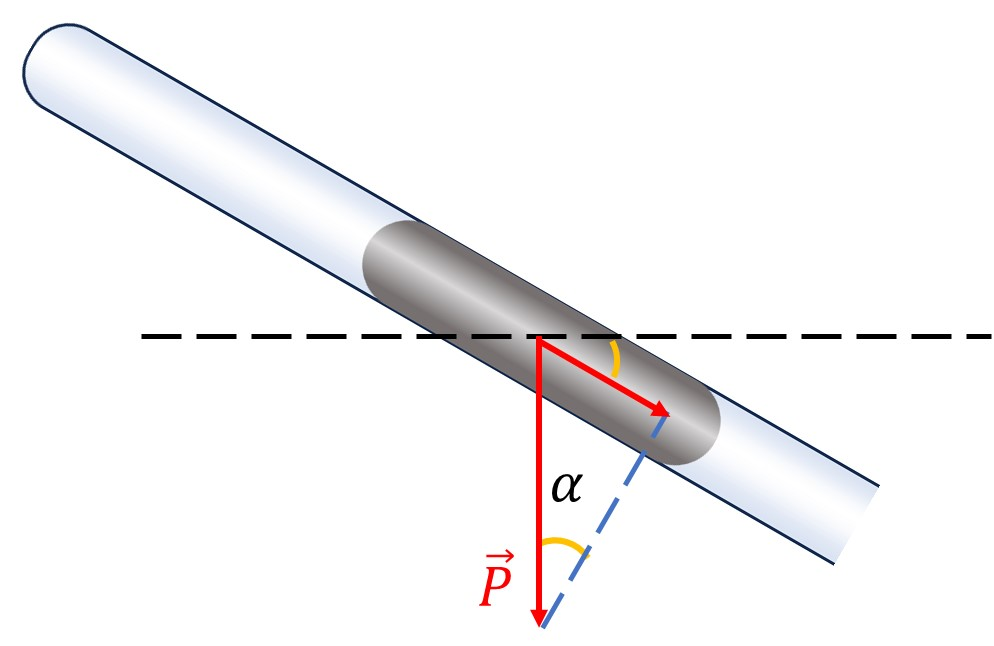
\includegraphics[width=1.0\linewidth]{../figs/VN12-Y24-PH-SYL-010-6}
	\end{center}
\end{minipage}
\begin{minipage}[l]{0.75\textwidth}
	\begin{center}
		\begin{tabular}{C{4cm} C{1.5cm} C{4.5cm}}
			\colorbox{yellow}{\textcolor{red}{\textbf{Trạng thái ban đầu}}} & $\xrightarrow[]{T=const}$ & \colorbox{yellow}{\textcolor{red}{\textbf{Trạng thái câu c}}}\\
			$p_0=\SI{750}{\milli\meter Hg}$ & &$p_c=p_0-d\sin\alpha=\SI{675}{\milli\meter Hg}$\\
			$V_0=\ell_0S$ & & $V_c=\ell_c S$
		\end{tabular}
	\end{center}
	Theo định luật Boyle:
	$$p_0V_0=p_cV_c$$
	$$\Leftrightarrow p_0\ell_0S=p_c\ell_cS$$
	$$\Rightarrow \ell_c=\dfrac{p_0\ell_0}{p_c}=\dfrac{\left(\SI{750}{\milli\meter Hg}\right)\cdot\left(\SI{144}{\milli\meter}\right)}{\SI{675}{\milli\meter Hg}}=\SI{160}{\milli\meter}.$$
\end{minipage}
\item Trường hợp ống đặt nghiêng góc $\alpha=\SI{30}{\degree}$ so với phương ngang, miệng ống ở trên:\\
\begin{minipage}[l]{0.25\textwidth}
	\begin{center}
		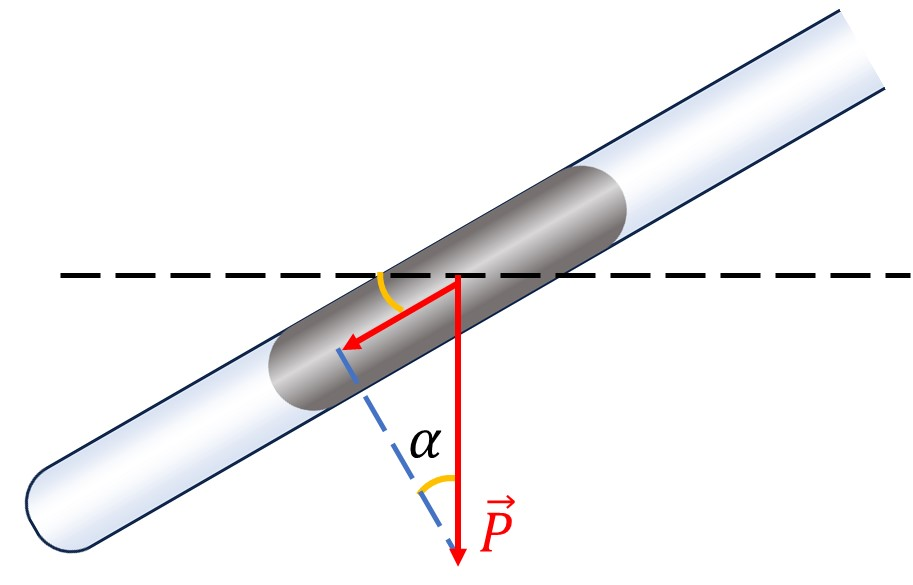
\includegraphics[width=1.0\linewidth]{../figs/VN12-Y24-PH-SYL-010-7}
	\end{center}
\end{minipage}
\begin{minipage}[l]{0.75\textwidth}
	\begin{center}
		\begin{tabular}{C{4cm} C{1.5cm} C{4.5cm}}
			\colorbox{yellow}{\textcolor{red}{\textbf{Trạng thái ban đầu}}} & $\xrightarrow[]{T=const}$ & \colorbox{yellow}{\textcolor{red}{\textbf{Trạng thái câu d}}}\\
			$p_0=\SI{750}{\milli\meter Hg}$ & &$p_d=p_0+d\sin\alpha=\SI{825}{\milli\meter Hg}$\\
			$V_0=\ell_0S$ & & $V_d=\ell_d S$
		\end{tabular}
	\end{center}
	Theo định luật Boyle:
	$$p_0V_0=p_dV_d$$
	$$\Leftrightarrow p_0\ell_0S=p_d\ell_dS$$
	$$\Rightarrow \ell_d=\dfrac{p_0\ell_0}{p_d}=\dfrac{\left(\SI{750}{\milli\meter Hg}\right)\cdot\left(\SI{144}{\milli\meter}\right)}{\SI{825}{\milli\meter Hg}}\approx\SI{131}{\milli\meter}.$$
\end{minipage}
\end{enumerate}
}}
\end{dang}
\begin{dang}{Giải được bài toán piston cân bằng}
	\viduii{3}{
	Một lượng không khí có thể tích $\SI{240}{\centi\meter^3}$ chứa trong một cylanh có piston đóng kín, tiết diện của piston là $\SI{24}{\centi\meter^2}$. Áp suất của không khí trong cylanh bằng áp suất không khí bên ngoài là $\SI{E5}{\pascal}$. Cần một lực tối thiểu bằng bao nhiêu để dịch chuyển piston một đoạn $\SI{2}{\centi\meter}$ theo chiều làm thể tích khí giảm? Bỏ qua ma sát giữa giữa piston và thành cylanh. Coi trong quá trình piston chuyển động thì nhiệt độ của không khí không thay đổi.
	\begin{center}
		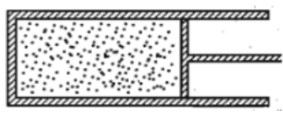
\includegraphics[width=0.25\linewidth]{../figs/VN12-Y24-PH-SYL-010-8}
	\end{center}
}
{\hide{
	\begin{center}
		\begin{tabular}{C{6cm} C{2cm} C{7cm}}
			\colorbox{yellow}{\textcolor{red}{\textbf{Trạng thái 1}}} & $\xrightarrow[]{T_1=T_2}$ & \colorbox{yellow}{\textcolor{red}{\textbf{Trạng thái 2}}}\\
			$p_1=\SI{E5}{\pascal}$ & &$p_2=?$\\
			$V_1=\SI{240}{\centi\meter^3}$ & & $V_2=\SI{240}{\centi\meter^3}-\left(\SI{24}{\centi\meter^2}\right)\cdot\left(\SI{2}{\centi\meter}\right)=\SI{192}{\centi\meter^3}$
		\end{tabular}
	\end{center}
Theo định luật Boyle:
$$p_1V_1=p_2V_2\Rightarrow p_2=\dfrac{p_1V_1}{V_2}=\dfrac{\left(\SI{100}{\kilo\pascal}\right)\cdot\left(\SI{240}{\centi\meter^3}\right)}{\SI{192}{\centi\meter^3}}=\SI{125}{\kilo\pascal}.$$
\begin{center}
	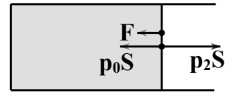
\includegraphics[width=0.25\linewidth]{../figs/VN12-Y24-PH-SYL-010-9}
\end{center}
Piston cân bằng khi:
$$p_2S=p_0S+F\Rightarrow F=\left(p_2-p_0\right)S=\left(\SI{125E3}{\pascal}-\SI{100E3}{\pascal}\right)\cdot\left(\SI{24E-4}{\meter^2}\right)=\SI{60}{\newton}.$$
}}

\viduii{3}
{Một bình hình trụ kín hai đầu có độ cao $h=\SI{40}{\centi\meter}$, được đặt nằm ngang, bên trong có một piston rất mỏng và có thể dịch chuyển không ma sát trong bình. Lúc đầu piston được giữ cố định ở chính giữa bình. Hai bên piston chứa cùng loại khí nhưng áp suất khí bên trái $\left(p_1\right)$ lớn gấp 3 lần áp suất khí chứa ở bên phải $\left(p_2\right)$. Piston và thành bình đều được làm từ vật liệu cách nhiệt. Khi thả để piston di chuyển tự do thì piston sẽ di chuyển một đoạn bao nhiêu, theo chiều nào?
\begin{center}
	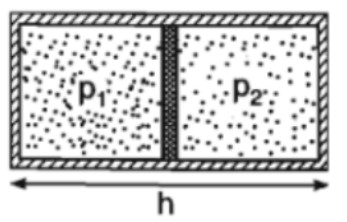
\includegraphics[width=0.25\linewidth]{../figs/VN12-Y24-PH-SYL-010-10}
\end{center}

}
{\hide{
	Vì áp suất khí bên trái lớn hơn áp suất khí bên phải nên khi được thả tự do piston sẽ di chuyển theo chiều từ trái sang phải.\\
	Piston di chuyển đến khi áp suất khí hai bên piston cân bằng. Gọi:
	\begin{itemize}
		\item $p$ là áp suất khí mỗi bên khi piston đạt trạng thái cân bằng;
		\item $x$ là độ dời của piston.
	\end{itemize}
	Áp dụng định luật Boyle cho khí ở mỗi vách ngăn khi vừa thả piston và khi piston cân bằng:
	$$pV=\text{const}\Rightarrow \begin{cases}
		p_1\cdot\dfrac{hS}{2}=p\left(\dfrac{h}{2}+x\right)S\\
		p_2\cdot\dfrac{hS}{2}=p\left(\dfrac{h}{2}-x\right)S\\
	\end{cases}\Rightarrow \dfrac{p_1}{p_2}=\dfrac{\SI{20}{\centi\meter}+x}{\SI{20}{\centi\meter}-x}=3\Rightarrow x=\SI{10}{\centi\meter}.$$

}}
\end{dang}
